%%
%% Copyright (c) 2010 Philipp Reh 
%%


\chapter{Parser}

Das \gtitool kann kontextfreie Grammatiken in verschiedene Parser konvertieren:
\begin{itemize}
\item Top-Down-Parser
\item LR0-Parser
\item SLR-Parser
\item LALR1-Parser
\item LR1-Parser
\end{itemize}

\section{Allgemeine Anzeige der Parser}
Zu jedem Parser wird links der aktuelle Fortschritt angezeigt, dessen Einträge
mindestens aus dem noch zu lesenden Wort, dem aktuellen Keller, und der
ausgeführten Aktion bestehen.
Ein Wort kann über das Menü "`Ausführen"' und "`Wort eingeben"' eingegeben werden. 
Die Nagivation für den Ablauf des Parsens ist gleich der Navigation eines Automaten.

\section{Top-Down-Parser}

Der deterministische Top-Down-Parser benutzt FOLLOW,
um seine möglichen Aktionen zu bestimmen, d.h. die Aktionstabelle besteht
aus Einträgen zu einem Terminalzeichen und einem Nichtterminalzeichen.
Ist solch ein Eintrag nicht leer, bedeutet dies, dass der Parser
die eingetragenen Produktion anwenden kann, falls er auf das entsprechende
Terminalzeichen stößt und das Nichtterminalzeichen oben im Keller liegt.
Terminalzeichen im Keller werden implizit gegen die der Eingabe aufgehoben.

\begin{figure}[h]
\begin{center}
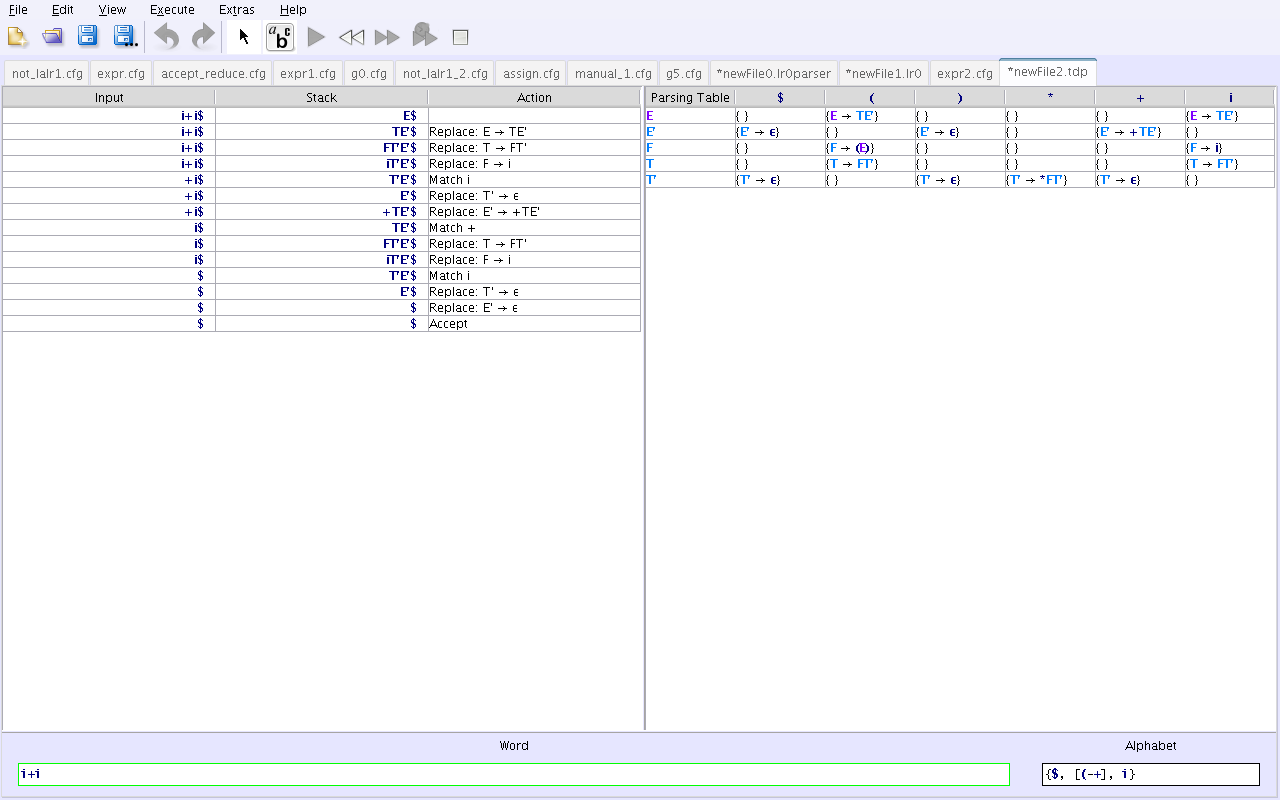
\includegraphics[width=12cm]{../images/tdp.png}
\end{center}
\end{figure}

\section{LR-Parser}

Die vier LR-Parser benutzen die entsprechenden ACTIONS-Funktionen,
um zu steuern, ob sie Shiften, Reduzieren oder akzeptieren müssen.

Die LR-Parser zeigen zusätzlich rechts unten die berechnete GOTO-Tabelle an.
Ebenso wird links zusätzlich der Zustandskeller angezeigt. Der oberste
Zustand auf dem Keller entspricht dem aktuellen Zustand.

\begin{figure}[h]
\begin{center}
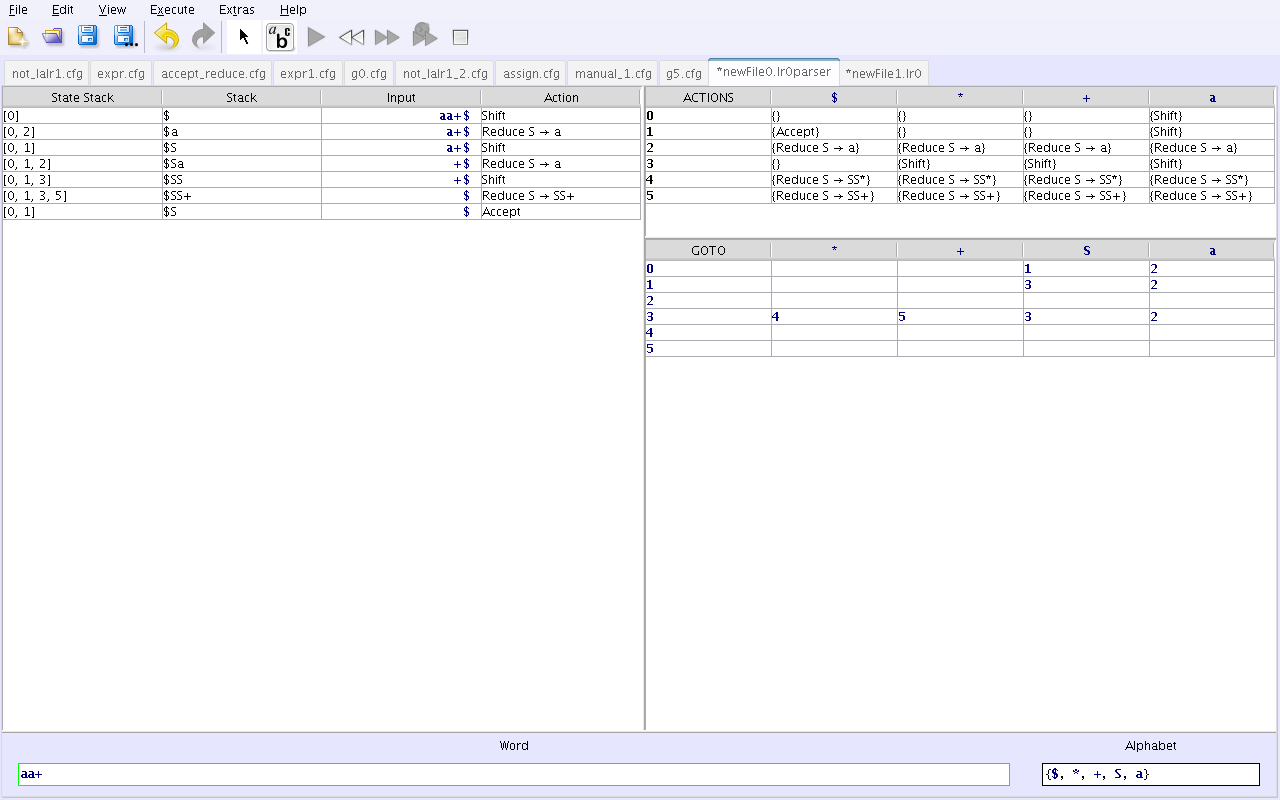
\includegraphics[width=12cm]{../images/lr.png}
\end{center}
\end{figure}
